\documentclass[10pt]{article}
\usepackage[margin=1in]{geometry}
\usepackage[T1]{fontenc}
\usepackage{lmodern}
\usepackage{microtype}
\usepackage{amsmath}
\usepackage{booktabs}
\usepackage{multirow}
\usepackage{graphicx}
\usepackage{xcolor}
\usepackage[numbers,sort&compress]{natbib}
\usepackage[colorlinks=true,linkcolor=blue!50!black,citecolor=blue!50!black,urlcolor=blue!50!black]{hyperref}
\usepackage{caption}
\captionsetup{font=small,labelfont=bf}

\newcommand{\pstale}{P(\text{stale})}

\title{The Stale Present: Video-Language Models Often Report\\the Previous State Instead of the Current One}
\author{%
  \textcolor{red}{[Author names --- TODO]}\\
  \textcolor{red}{[Affiliation --- TODO]}\\
  \texttt{\textcolor{red}{[email --- TODO]}}
}
\date{}

\begin{document}
\maketitle

\begin{abstract}
We ask open video-language models (VLMs) a simple question: \emph{what is shown at the end of the video?} The answer is clearly visible in the final frames, and every model answers it almost perfectly when given only the last frame. Given the whole video, however, many models answer with the \emph{previous} state of the scene. We call this failure the \emph{stale present}. On synthetic scenes with four earlier layouts and a 0.5\,s final state, accuracy of eight open models ranges from 0.30 to 0.80, against 1.00 from the last frame alone. On real chess games, Qwen3-VL-8B names the captured piece instead of the capturing one in 59--78\% of trials. Using controlled stimuli and preregistered tests, we find four things. (i) The effect is driven by the number of earlier states of the same kind and by how briefly the final state is shown; frame rate does not matter. (ii) It is a mid-layer retrieval by the question tokens: blocking the text positions' attention to the previous state in a narrow band of middle layers removes most stale answers in Qwen3-VL-8B and Gemma-3-12B. (iii) The same holds on real footage once a clean previous state is present; there, real and rendered frames give effects of the same size. (iv) A training-free contrastive decoding that subtracts the score of the video truncated before the last change removes the stale answers. However, it never beats simply reading the last frame on pure present-state questions; it helps only when the question also needs the history. We also report the limits of the phenomenon. The newest model we tested, Qwen3.6-27B, is immune (0.98--1.00). In natural real-world shuffling videos, the effect of history is robust (about 10 points) but only some models concentrate their errors on the previous state. We therefore present the stale present as a documented, mechanistically localized failure of current mid-sized video VLMs, not as a universal property.
\end{abstract}

\section{Introduction}

A video assistant is often asked about the \emph{current} state of a scene: whether a drawer is open now, where an object ended up, which piece now stands on a chess square. Answering needs two things: seeing the last frames and knowing that they are the last ones. Video benchmarks usually conflate these two with memory and reasoning. We isolate them with a deliberately easy question whose answer is plainly visible at the end of the clip, and a matched control that shows the model only the final frame.

The failure we study is easy to state. A model reads the last frame correctly when it sees that frame alone, yet with the full video it names the state that came \emph{just before} (Figure~\ref{fig:models}). The error is not random: when a model is wrong, it almost always chooses the immediately preceding state. We call this the \emph{stale present}.

This paper is an analysis paper. Most tests were preregistered in a versioned file before the data were generated or the models were run. We report failed predictions and retracted interpretations alongside the supported ones. Our contributions are:
\begin{itemize}
  \item \textbf{A controlled demonstration} (\S\ref{sec:phenomenon}) across twelve open VLMs from five families, on synthetic layouts and on real chess games (MET-Bench~\cite{cohen2026metbench}). Every comparison is paired with a last-frame control, and the real-footage comparisons also with a same-pipeline ``frozen video'' control.
  \item \textbf{What drives it} (\S\ref{sec:drivers}). The effect needs at least two states of the same kind before the final one, grows with their number, and shrinks with the final dwell. In a factorial test, going from 1 to 4 prior states adds 0.24 to the last-frame-minus-video gap, longer prior states add 0.07, and frame rate adds nothing.
  \item \textbf{Where it happens} (\S\ref{sec:mechanism}). Blocking the question tokens' attention to the previous state inside a narrow band of middle layers (relative depth 0.4--0.7) removes most stale answers in two models, and fails in a third. Answer-position ``recency heads'' found by correlation are not causal.
  \item \textbf{Real footage} (\S\ref{sec:real}). In natural shuffling videos from Perception Test~\cite{patraucean2023perception}, history costs about 10 points of accuracy over a frozen-video control. When a clean, well-held previous state is shown, the stale rate rises by 0.10 on real frames, as much as on rendered tiles, and the same mid-layer masking removes it.
  \item \textbf{A fix and its boundary} (\S\ref{sec:fix}). Present-contrastive decoding (PCD) removes the stale answers. It is useful only on questions that need the history as well as the present; for pure present-state questions, reading the last frame is as good.
\end{itemize}

We are explicit about the limits (\S\ref{sec:limits}). The newest model we tested is immune; sample sizes are 50--100 per cell; and the strongest real-footage effect uses a spliced timeline.

\begin{figure}[t]
  \centering
  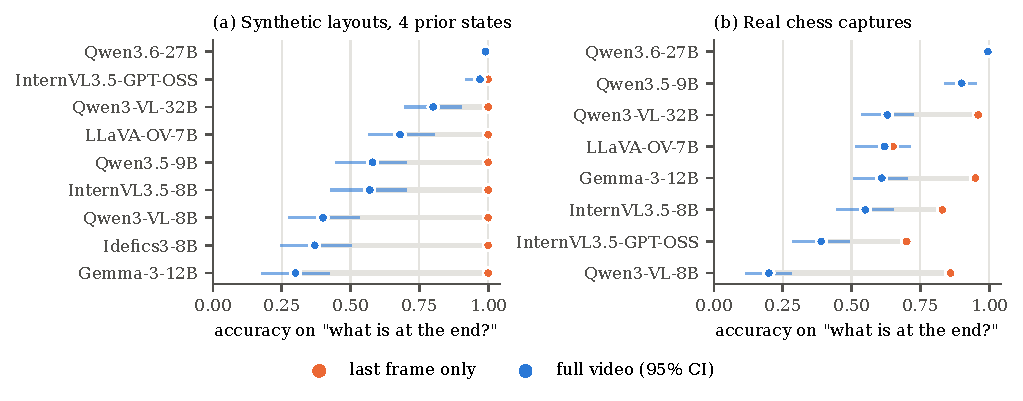
\includegraphics[width=\linewidth]{figs/fig_models.pdf}
  \caption{\textbf{The stale present across models.} Accuracy on ``what is at [position] at the very end?'' when the model sees the last frame only (orange) or the full video (blue, 95\% bootstrap CI). (a) Synthetic colored layouts with four prior layouts and a 0.5\,s final layout ($n=60$ per model). (b) Real chess games, capture squares, one prior move, 0.5\,s final position ($n=100$). For Qwen3.6-27B only the video condition was run. In (b), Idefics3-8B is omitted because it cannot read the board (last-frame accuracy 0.48).}
  \label{fig:models}
\end{figure}

\section{Related work}

\paragraph{State tracking in video VLMs.} VET-Bench~\cite{liu2026shellgame} shows that VLMs are at chance on the shell game and that grounded trajectory reasoning fixes it. MET-Bench~\cite{cohen2026metbench} finds a large gap between text-based and image-based entity tracking in chess and shell games. TOC-Bench~\cite{chen2026tocbench} and StateTrace~\cite{han2026statetrace} test object identity and hidden-state persistence under occlusion. Event bookkeeping at high frequencies fails as well~\cite{baskar2026lowfreq}. Our question is simpler than all of these: the answer is visible, nothing is occluded, and no tracking is needed.

\paragraph{Last-frame shortcuts and temporal grounding.} Several works note that single frames often match or beat full clips on video QA~\cite{ok2025tempcore}. EgoIntent~\cite{pan2026egointent} reports that the last boundary frame outperforms the ordered clip for several models. VLX-VR~\cite{li2026vlxvr} observes models being drawn to a later salient event instead of the state a question asks for. We study the reverse direction, an earlier state overriding the current one. We control for image quality with a frozen-video condition, and we localize the effect inside the model.

\paragraph{Contrastive decoding.} Contrastive decoding~\cite{li2023cd} and its visual variants~\cite{leng2024vcd} subtract the scores of a degraded input. SEASON~\cite{wu2025season} builds temporally homogenized negatives for video. Our PCD uses the video truncated before the last detected change as the negative, which targets exactly the stale state. We find that its value is narrower than such methods usually claim.

\paragraph{Localizing retrieval by attention blocking.} We follow the attention-knockout methodology of \citet{geva2023dissecting}: we block attention edges from text positions to chosen visual tokens in chosen layers and measure the change in the answer.

\section{Setup}
\label{sec:setup}

\paragraph{Models.} We evaluate the following models locally in bf16:
\begin{itemize}
  \item Qwen3-VL 2B/4B/8B/32B-Instruct~\cite{bai2025qwen3vl}, Qwen3.5-9B, Qwen3.6-27B and Qwen2.5-VL-7B~\cite{bai2025qwen25vl}, all with native video input;
  \item LLaVA-OneVision-7B~\cite{li2024llavaov} and InternVL3.5-8B~\cite{wang2025internvl35}, with video input;
  \item Gemma-3-12B~\cite{gemma2025gemma3}, Idefics3-8B~\cite{laurencon2024idefics3} and InternVL3.5-GPT-OSS-20B-A4B, with frames given as a numbered image list (``Frame $i$:''), at most 32 uniformly sampled frames, always including the last.
\end{itemize}
LLaVA-NeXT-Video-7B was excluded because it could not read the final frame (last-frame accuracy 0.22--0.74).

\paragraph{Questions and scoring.} Every question is multiple choice with three options: the correct final content, the content of the previous state at the queried place (the \emph{stale} option), and one other content present in the video. The option order is shuffled. We score the argmax over the option-letter logits right after the generation prompt, with thinking disabled. We report accuracy and \pstale, the rate of choosing the stale option.

\paragraph{Controls.}
\begin{itemize}
  \item \emph{Last frame}: the final frame alone, as a single image, with the same question.
  \item \emph{Frozen video} (real footage only): the final frame repeated for the length of the clip and fed through the same video pipeline. It keeps the video path's resolution and temporal merging but removes the history.
\end{itemize}
The difference between the frozen video and the real video isolates the effect of history.

\paragraph{Stimuli.}
\begin{itemize}
  \item \textbf{Synthetic layouts.} Colored cups or disks on a table, rendered in 2D at 4\,fps. Static layouts change abruptly; there is no motion and no occlusion. A reveal layout is followed by $m$ further layouts, each held 1\,s, and the last one is held $D_\text{fin}$.
  \item \textbf{Real chess.} Board positions from real MET-Bench game records, rendered with glyphs, $m\in\{1,3\}$ prior moves, $D_\text{fin}\in\{0.5,2\}$\,s. On capture squares, the stale answer is the captured piece.
  \item \textbf{Word tiles.} Letter tiles spelling the orders of the real Perception Test word-shuffle videos, used for the factorial study.
  \item \textbf{Real footage.} Perception Test letter-shuffling videos (via MVBench~\cite{li2024mvbench}) with the official per-second letter boxes (\S\ref{sec:real}).
\end{itemize}

\paragraph{Statistics.} We use paired bootstrap 95\% CIs (10{,}000 resamples; stratified by model when pooling) and exact McNemar tests. The CI table for all fix experiments is Holm-corrected within each difference column. Each preregistration states a threshold, and we call a prediction supported only if the point estimate meets it. Two real-footage tests (\S\ref{sec:real}) had CIs clearly above zero but point estimates of 0.096 and 0.097 against a threshold of 0.10; we report them as failed.

\section{The phenomenon}
\label{sec:phenomenon}

\paragraph{Main result.} Figure~\ref{fig:models} shows the core comparison. On synthetic layouts with $m=4$ and $D_\text{fin}=0.5$\,s, every model answers the last frame alone perfectly, yet video accuracy is 0.30 (Gemma-3-12B) to 0.80 (Qwen3-VL-32B). Qwen3-VL-2B and 4B score 0.42 and 0.45. The errors are stale: for Qwen3-VL-8B and Qwen3.5-9B with $m=2$, 52--59 of 55--70 errors pick the immediately preceding layout. On real chess captures, Qwen3-VL-8B reads the final board at 0.86 but answers from the video at 0.20, choosing the captured piece in 78\% of trials. The paired last-frame minus video differences are highly significant for Qwen3-VL-8B on every chess cell (McNemar $p\le 10^{-7}$ after Holm correction).

\paragraph{Not every model, and not the newest.} Qwen3.6-27B scores 0.98--1.00 on every synthetic and chess cell. InternVL3.5-GPT-OSS is almost immune on synthetic layouts (0.97) but not on chess (0.39, with \pstale{} of 0.57). Qwen3.5-9B shows no gap on the easiest chess cell. Within the Qwen3-VL family, the 32B model is much less affected than the 2B--8B models.

\section{What drives the stale present}
\label{sec:drivers}

\paragraph{Final dwell.} In the first test, three layouts followed the reveal, with the dwells of the last two varied independently (Qwen3-VL-8B and Qwen3.5-9B, $n=60$ per cell). Accuracy rises from 0.45--0.58 at $D_\text{fin}=0.5$\,s to 0.83--0.93 at 4\,s. The dwell of the previous layout has only a small effect.

\paragraph{Same-kind prior states.} When the only earlier layout is the visually distinct reveal (cups lifted, ball visible), the present is reported correctly even at 0.5\,s (0.92--1.00). One additional cups-down layout halves accuracy (0.48--0.57). Showing a single initial layout for 2.5--5\,s before a 0.75\,s final layout does not produce the effect (0.87--0.98). The model does not simply weight states by how long they were shown. It confuses \emph{which of several similar changes was the last}.

\paragraph{Minimal displays.} A single digit or a single ball that jumps between positions does not trigger the effect (0.92--1.00). Three colored disks do, when asked ``where is the red disk?'' (Qwen3-VL-8B 0.50, Qwen3.5-9B 0.48). A single disk also triggers it when the question is keyed by position (``what is on the left?''): Qwen3-VL-8B 0.54, Qwen3-VL-32B 0.46. The stale present thus needs either several objects or a position-keyed query.

\paragraph{Not a tokenization artifact.} Qwen models merge two frames into one temporal token group. All state changes in our videos fall on group boundaries, so no group mixes old and new frames. Feeding the same frames as a timestamped image list weakens the effect (Qwen3-VL-8B, $m=2$: 0.57$\to$0.85) but does not remove it; \pstale{} stays at 0.12--0.23. Models that take image lists natively (Gemma-3, Idefics3) show the effect in full (Figure~\ref{fig:models}a).

\paragraph{Factorial test of the timeline.} On letter-tile renderings of the real word-shuffle items, we crossed three factors for five models ($n=67$ each): the number of prior states $m\in\{1,4\}$, the dwell per prior state $\in\{1,4\}$\,s, and the frame rate $\in\{2,4\}$\,fps. The final state was held 0.5\,s. Figure~\ref{fig:timeline} shows the result. The main effect of $m$ on the last-frame minus video gap is $+0.240$ [0.181, 0.300] for position questions and $+0.236$ [0.187, 0.284] for order questions. The dwell adds $+0.069$ [0.046, 0.094]; frame rate adds $-0.011$ [$-0.027$, 0.004]. \pstale{} follows the same pattern. At $m=4$, every model shows a position-question gap of 0.42--0.60, including Qwen3.5-9B, whose gap at $m=1$ is only about 0.04.

\begin{figure}[t]
  \centering
  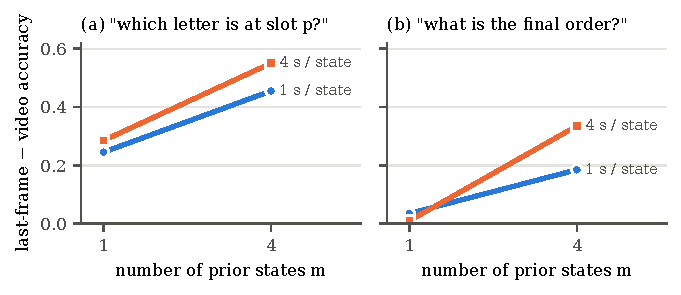
\includegraphics[width=0.62\linewidth]{figs/fig_timeline.pdf}
  \caption{\textbf{More prior states, and longer ones, make the present staler.} Pooled last-frame minus video accuracy (5 models, $n=67$ each; averaged over 2 and 4\,fps, which had no effect). The final state is held 0.5\,s. (a) Position questions. (b) Order questions, which need all letters: with a single prior state they show no gap.}
  \label{fig:timeline}
\end{figure}

\paragraph{Other interventions.} Appending the final frame as an extra image after the video only partly helps (Qwen3-VL-8B, $m=4$: 0.40$\to$0.65, against 1.00 for the last frame alone). The video overrides an explicitly given present. Chain-of-thought is inconsistent: it helps some cells, hurts others, and often hallucinates intermediate layouts.

\section{Where the stale answer is retrieved}
\label{sec:mechanism}

\paragraph{Attention is not recency-weighted, and correlated heads are not causal.} In Qwen3-VL-8B, the final and the previous layouts receive similar attention from the answer position (final share 0.46--0.53). A few heads in layers 24--27 attend to the final layout more on correct trials (0.76--0.79) than on stale ones (about 0.50). We preregistered a causal test: suppress the previous layout for these heads at the answer position. It had no effect, so the prediction was falsified.

\paragraph{Band masking.} We instead block \emph{all} text positions after the video from attending to the previous state's visual tokens, only within a chosen band of layers. The mask is applied inside the attention function; visual positions are untouched. Figure~\ref{fig:layers}a shows the drop in \pstale{} per band.
\begin{itemize}
  \item \textbf{Qwen3-VL-8B} (36 layers; dwell data, $D_\text{fin}\le 1$\,s). Masking in all layers raises accuracy from 0.60 to 0.80 and lowers \pstale{} from 0.33 to 0.075. Layers 18--26 alone give the full effect (0.81, 0.08). Layers 0--8 and 27--35 do nothing. Masking only the last token barely helps (0.60$\to$0.63), so the retrieval is spread over the question tokens.
  \item \textbf{Gemma-3-12B} (48 layers; preregistered, $n=320$). Masking in all layers raises accuracy from 0.547 to 0.709 (McNemar 54:2, $p=4\times10^{-14}$). The single band 18--23 gives 81\% of this gain, and the 8 global-attention layers alone give about 95\%. Masking the final state instead collapses accuracy to 0.138 (\pstale{} 0.728). Masking earlier states changes accuracy by only $-0.03$.
  \item \textbf{Idefics3-8B.} All-layer masking gives only 0.45$\to$0.50, so the preregistered prediction fails.
  \item \textbf{Qwen2.5-VL-7B.} Partial: the best band is 14--20 of 28, but \pstale{} drops only from 0.37 to 0.28.
\end{itemize}
In the two models where masking works, the stale answer is fetched by the question tokens from the previous state's visual tokens in middle layers. The remaining gap to the last-frame control (0.81 vs 1.00 in Qwen3-VL-8B) presumably sits in the visual token stream itself. For Idefics3 and Qwen2.5-VL, more of the effect seems to sit there.

\begin{figure}[t]
  \centering
  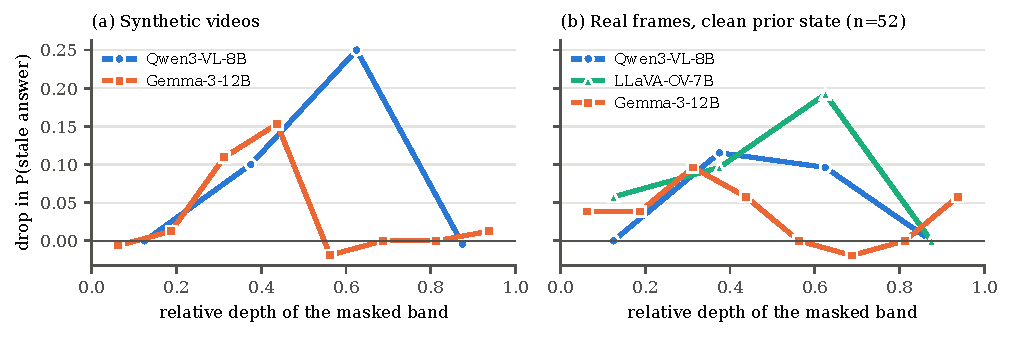
\includegraphics[width=\linewidth]{figs/fig_layers.pdf}
  \caption{\textbf{The stale answer is retrieved in middle layers.} Drop in \pstale{} when the question tokens are blocked from the previous state's visual tokens within one band of layers (x: band center divided by the number of layers). (a) Synthetic videos: Qwen3-VL-8B ($n=240$, $D_\text{fin}\le1$\,s) and Gemma-3-12B ($n=320$). (b) Real frames with a clean prior state held 4\,s (\S\ref{sec:real}; $n=52$ per model). Shallow and deep bands have no effect.}
  \label{fig:layers}
\end{figure}

\section{Real footage}
\label{sec:real}

\paragraph{Natural videos: history costs accuracy, but errors are not reliably stale.} We used the Perception Test videos in which letters are shuffled and the question asks for the final word order. A preregistered pilot (6 models, 79 questions) failed: the pooled last-frame minus video difference was $+0.04$ [$-0.00$, 0.08], against a threshold of 0.10. PCD also failed, because its change detector fires on hand and camera motion. We then diagnosed the failure step by step:
\begin{itemize}
  \item \textbf{Final dwell is not the cause.} Cropping to the letters and cutting the clip 0.5\,s or 2\,s after the last change did not help ($+0.01$).
  \item \textbf{Real shuffles are multi-step.} Reconstructed from the per-second letter boxes, 42 of 74 videos contain 3--13 changes, and the initial order is the true previous state in only 10 of 73. The pilot's ``stale option'' was therefore mostly the wrong target.
  \item \textbf{History has a robust cost.} With the question targeting the reconstructed previous state, and with a frozen-video control that goes through the same pipeline, history costs $+0.097$ [0.051, 0.144] accuracy (position questions, 6 models). The pipeline itself costs only $+0.025$ (n.s.).
  \item \textbf{But the errors are not reliably stale.} \pstale{} rises from the frozen video to the real video only for InternVL3.5-8B (0.18$\to$0.31) and LLaVA-OV-7B (0.21$\to$0.31).
\end{itemize}
A further check explained this. Most reconstructed ``previous states'' are transit orders captured while a hand carries a letter. Counting only \emph{resting} states (no letter centroid moves more than $0.25\times$ the letter height between adjacent samples), 45 of 73 videos have exactly one resting prior state, and 22 have none. Natural shuffles therefore offer essentially $m=1$, the regime in which even synthetic videos show a small effect (Figure~\ref{fig:timeline}).

\paragraph{Real frames on a controlled timeline.} For the 52 videos with a resting prior state, we built clips at 2\,fps: a real frame of that state held 4\,s, then the real final frame for 0.5\,s. The same timeline was also rendered with letter tiles. Table~\ref{tab:ag} shows the result. History raises \pstale{} by $+0.103$ [0.054, 0.151] on real frames and by $+0.106$ on tiles, so the preregistered prediction on \pstale{} is supported. The accuracy prediction failed narrowly ($+0.096$ against the threshold of 0.10). The domain difference is $+0.035$ [$-0.022$, 0.093]. Real images do not block the stale present; natural timelines rarely set it up. The largest real-frame effects are in Qwen3-VL-8B (0.21$\to$0.40) and LLaVA-OV-7B (0.17$\to$0.42). Order questions show no effect in either domain, as expected at $m=1$.

\begin{table}[t]
  \centering
  \small
  \caption{\textbf{Real frames vs.\ rendered tiles on the same timeline} (prior state 4\,s, final 0.5\,s; 6 models $\times$ 52 items, position questions). Frozen: the final frame repeated through the video pipeline.}
  \label{tab:ag}
  \begin{tabular}{lccccc}
    \toprule
    & last frame & frozen & video & frozen $-$ video & \pstale: frozen $\to$ video \\
    \midrule
    Real frames & 0.72 & 0.70 & 0.60 & $+0.096$ [0.048, 0.144] & 0.22 $\to$ 0.33 \\
    Rendered tiles & 0.92 & 0.94 & 0.80 & $+0.131$ [0.096, 0.170] & 0.04 $\to$ 0.15 \\
    \bottomrule
  \end{tabular}
\end{table}

\paragraph{The same mid-layer retrieval on real frames.} We applied band masking to these real clips (preregistered; Figure~\ref{fig:layers}b, Table~\ref{tab:ah}). In all three models, the unmasked answers reproduced the earlier run exactly.
\begin{itemize}
  \item \textbf{Qwen3-VL-8B.} Blocking the previous state in all layers lowers \pstale{} from 0.40 to 0.25 (9:1, $p=0.02$). This is close to its no-history level of 0.21.
  \item \textbf{LLaVA-OV-7B.} \pstale{} falls from 0.42 to 0.21 (12:1, $p=0.003$), and the single band 14--20 of 28 gives almost all of it.
  \item \textbf{Gemma-3-12B.} The real-frame effect is small; only its global layers give a significant drop.
\end{itemize}
We had predicted that Qwen3-VL-8B's synthetic band (18--26) would also be the best band on real frames. It recovered 62\% of the effect, but the adjacent band 9--17 did slightly better, by one item. The localization thus holds at the level of ``middle layers'' but is broader and slightly shallower on real frames.

\begin{table}[t]
  \centering
  \small
  \caption{\textbf{Band masking on real frames} ($n=52$ per model). \pstale{} (accuracy in parentheses). Counts: items that stopped / started being stale; McNemar $p$.}
  \label{tab:ah}
  \begin{tabular}{llll}
    \toprule
    mask & Qwen3-VL-8B & LLaVA-OV-7B & Gemma-3-12B \\
    \midrule
    none & 0.40 (0.58) & 0.42 (0.58) & 0.35 (0.56) \\
    previous state, all layers & 0.25 (0.69); 9:1, $p$=.02 & 0.21 (0.73); 12:1, $p$=.003 & 0.25 (0.63); 6:1, $p$=.13 \\
    best single band & 0.29 (0.65), L9--17 & 0.23 (0.69), L14--20 & 0.23 (0.63), global layers \\
    final state, all layers & 0.83 (0.10) & 0.75 (0.17) & 0.52 (0.27) \\
    \midrule
    frozen video (no history) & 0.21 & 0.17 & 0.29 \\
    \bottomrule
  \end{tabular}
\end{table}

\section{A training-free fix and where it stops working}
\label{sec:fix}

\paragraph{Method.} We first locate the last change $t_c$ with a pixel change detector. \emph{Present-contrastive decoding} (PCD) then scores each option as
\[
s(a) = \log p(a \mid \text{video}) - \alpha \log p(a \mid \text{video}_{<t_c}), \qquad \alpha = 1 \text{ (preregistered)}.
\]
The second term measures what the model would answer from the past alone, so the stale option is penalized. For Qwen3-VL we also test \emph{change-point masking} (CPM), which applies the mid-layer mask of \S\ref{sec:mechanism} to all visual tokens before $t_c$.

\paragraph{Pure present-state questions: no better than the last frame.} PCD removes most stale answers (Table~\ref{tab:fix}). For example, Qwen3-VL-8B on chess goes from 0.20 to 0.84, with \pstale{} from 0.78 to 0.04, and CPM performs similarly. But reading the last frame alone is just as good. Across 88 model$\times$cell comparisons (9 models), PCD is never significantly above the last frame after Holm correction. In 8 of them it is significantly below, e.g.\ Gemma-3 on layouts ($-0.27$) and Idefics3 on layouts ($-0.25$). If a question asks only about the present, the right fix is to answer from the last frame.

\paragraph{Questions that need the history.} PCD earns its keep when the answer must combine history and present. We asked, on real chess exchanges: ``What is \emph{now} on the square where the first move landed?'' The question does not name the stale answer. The last frame alone cannot identify the square, and the video alone answers stale. PCD improves over the last frame by $+0.29$ to $+0.47$ for Qwen3-VL-8B/32B, Qwen3.5-9B and InternVL3.5-8B (Holm-corrected $p\le 0.007$ in both dwell cells). At a 0.5\,s final dwell it also helps Gemma-3 ($+0.35$) and InternVL3.5-GPT-OSS ($+0.36$). It does not help LLaVA-OV or Idefics3. A disk version of the same question fails for every model and method (at most about 0.6): the models cannot retrieve the initial position either.

\paragraph{Robustness and failures.}
\begin{itemize}
  \item \textbf{The change point must be estimated.} Truncating a fixed $\Delta$ seconds hurts whenever $\Delta$ is shorter than the final dwell (InternVL3.5, 2\,s dwell: 0.63$\to$0.35).
  \item \textbf{Noise.} Under simulated camera noise, the pixel detector finds only 19 of 520 change points. A jitter-compensated detector (brightness normalization and $\pm3$\,px alignment; threshold set on a disjoint development set) restores the gains.
  \item \textbf{Real footage.} On natural video, hand and camera motion make the detector place the last change near the end of the clip (median 98\% of its length). PCD then fails.
  \item \textbf{Questions that name the stale item.} PCD is harmful when the question itself names the stale item (one cell fell from 0.82 to 0.05).
  \item \textbf{Noise amplification.} It can amplify noise in a model that ignores the input: Idefics3's single-ball control fell from 0.44 to 0.04.
\end{itemize}

\begin{table}[t]
  \centering
  \small
  \caption{\textbf{Training-free fixes.} Accuracy: last frame / video / PCD ($\alpha=1$). Chess and layouts ($m=4$) with $D_\text{fin}=0.5$\,s. History questions: ``what is now on the square where the first move landed?'', $D_\text{fin}=2$\,s, $n=100$. The last-frame value there is unpaired.}
  \label{tab:fix}
  \begin{tabular}{lccc}
    \toprule
    model & chess captures, $m=1$ & layouts, $m=4$ & history question (chess) \\
    \midrule
    Qwen3-VL-8B & 0.86 / 0.20 / 0.84 & 1.00 / 0.40 / 0.87 & 0.38 / 0.51 / \textbf{0.82} \\
    Qwen3-VL-32B & 0.96 / 0.63 / 0.98 & 1.00 / 0.80 / 0.98 & 0.46 / 0.50 / \textbf{0.88} \\
    Qwen3.5-9B & 0.90 / 0.90 / 0.98 & 1.00 / 0.58 / 0.88 & 0.41 / 0.70 / \textbf{0.88} \\
    InternVL3.5-8B & 0.83 / 0.55 / 0.76 & 1.00 / 0.57 / 0.87 & 0.39 / 0.63 / \textbf{0.78} \\
    Gemma-3-12B & 0.95 / 0.61 / 0.93 & 1.00 / 0.30 / 0.73 & 0.45 / 0.45 / \textbf{0.64} \\
    \bottomrule
  \end{tabular}
\end{table}

\section{Limitations and discussion}
\label{sec:limits}

\paragraph{The newest model is immune.} Qwen3.6-27B shows no stale present on any of our tests. Qwen3-VL-32B is much less affected than the 8B model, and InternVL3.5-GPT-OSS is almost immune on synthetic layouts. We did not test closed frontier models. The stale present may therefore be a property of current mid-sized open models that newer training already removes, rather than a lasting limitation. We think the controlled measurements, the timeline factors and the localized retrieval are still useful. They give a concrete test for new models, a diagnosis for the models that fail, and a warning for benchmark design: a clip whose final state is short and preceded by similar states can penalize a model for retrieval, not for perception.

\paragraph{Scale and realism.} Most cells have $n=50$--100, and the real-frame experiments have 52 items per model. Band-level comparisons within a model differ by only a few items and should not be read as layer-exact. Our synthetic scenes are clean 2D renders, and the chess boards are rendered from real game records. The strongest real-footage effect comes from a spliced timeline. In natural videos we find a robust cost of history but not a reliable preference for the previous state.

\paragraph{Preregistration.} Hypotheses and thresholds were written into a versioned file before each experiment. We did not use an external registry, so the ordering is documented only by our own records. Several analyses are explicitly exploratory: the non-Qwen replications of the fixes, the band splits in the natural-video diagnosis, and the global-layer finding in Gemma-3.

\section{Conclusion}

Asked what a video shows at its end, many current open video VLMs answer with what it showed just before. The failure grows with the number of similar earlier states and with a brief final state, and it does not depend on frame rate. It is produced by a mid-layer retrieval from the question tokens to the previous state's visual tokens, and it can be removed at inference time. It appears on real frames as strongly as on rendered ones once a clean previous state is present. The newest model we tested does not show it. For pure present-state questions, the last frame is the strongest baseline, and any fix should be compared against it.

\paragraph{Reproducibility.} Code, stimulus generators and the preregistration file will be released at \textcolor{red}{[URL --- TODO]}.

\bibliographystyle{plainnat}
\bibliography{refs}

\end{document}
